

\documentclass[25pt,a0paper, portrait]{tikzposter}
\usepackage[utf8]{inputenc}
\usepackage{xcolor}
\usepackage{graphicx,mwe}
\usepackage{filecontents}
\usepackage{lipsum}
\usepackage{tikz}
\usepackage{multicol}
\usepackage{adjustbox}
\usepackage{blindtext}
\usepackage{comment}


 \makeatletter
\def\TP@titlegraphictotitledistance{-6cm}
\settitle{ \centering \vbox{
		\@titlegraphic \\ [\TP@titlegraphictotitledistance] 
		\centering
		\color{titlefgcolor} 
		{\bfseries \Huge \sc \@title \par}
		\vspace*{1em}
		{\huge \@author \par}
}}
\makeatother

\setlength{\columnsep}{2cm}
 
\title{Schrittmotor Demonstrator}
\author{C. Crety, H. Mey, J. Perewersenko}
\titlegraphic{\includegraphics[height=6.5cm]{images/logo_hs_technik}
	\hfill
\includegraphics[height=6.5cm]{images/logo}
}
 
 
\usetheme{Desert}
 
\begin{document}

 
\maketitle

\begin{columns} 
	
	\column{0.36}
	{
		\colorlet{blocktitlebgcolor}{blue}
		\block{Projektbeschreibung}
		{
			Ziel des Projektes war es, einen Schrittmotor an einem CNC-Fräs- und Graviertisch als Demonstrator für die Funktionsweise eines Schrittmotor in Betrieb zu nehmen. Die Ansteuerung des Schrittmotors erfolgt über einen Arduino Nano 33 BLE Sense in Kombination mit einem Motortreiber vom Typ DRV8825. Über einen Dreh-Encoder können verschiedene Geschwindigkeitsstufen eingestellt werden, welche den Schrittmotor somit in verschiedenen Drehzahlen betreiben. 
			
			Zur Überwachung der tatsächlichen Geschwindigkeit wurde ein Geschwindigkeitssensor des Typs LM393 integriert. Die gemessene Geschwindigkeit wird auf einem OLED-Display ausgegeben, somit kann man die gemessene mit der eingestellten Geschwindigkeit vergleichen. 
			
			Das Projekt demonstriert damit die grundlegenden Steuerungs- und Messtechniken im Zusammenhang mit Schrittmotoren.
		}
		\block{CNC-Tisch}
		{
			Als Basis für dieses Projekt dient eine CNC-Fräs- und Graviermaschine, welche für Gravurarbeiten auf Materialien wie Holz, Kunststoffen oder Aluminium eingesetzt werden kann. 
			
			Die Maschine besitzt drei Schrittmotoren vom Typ NEMA 17, die drei Achsen antreiben. Außerdem gibt es einen Spindelmotor, der den Fräser antreiben kann. In diesem Projekt wird nur einer der drei Schrittmotoren betrieben. Die CNC-Fräs- und Graviermaschine verfügt zudem über eine integrierte Steuerplatine. In diesem Projekt wird diese jedoch nicht verwendet, da die Motorsteuerung über einen Arduino Nano 33 BLE Sense erfolgt.
		}
	}


	\column{0.64}
	{
		\colorlet{blocktitlebgcolor}{blue}
		\block{Elemente auf der Frontblende}
		{

					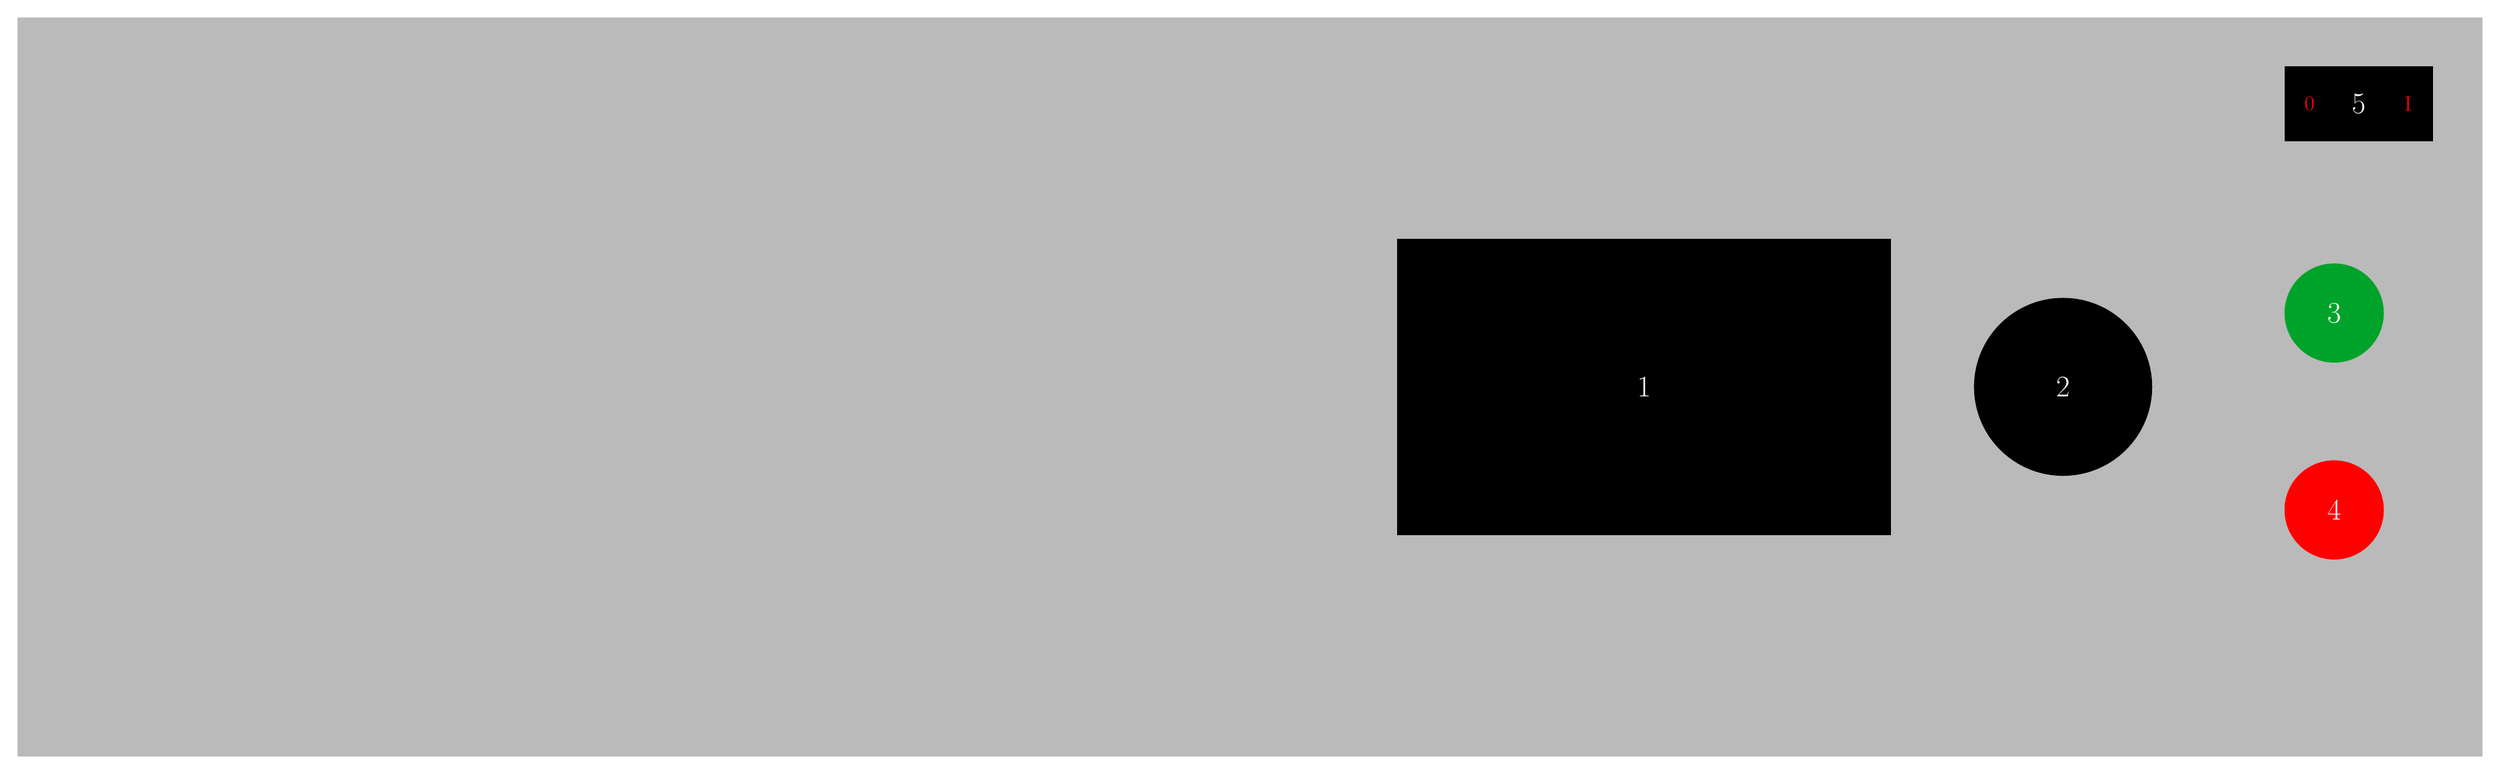
\begin{tikzpicture}
						\tikzstyle{every node}=[font=\LARGE]
						\draw [ color={rgb,255:red,186; green,186; blue,186} , fill={rgb,255:red,186; green,186; blue,186}] (0,15) rectangle (50,0);
						\draw [ fill={rgb,255:red,0; green,0; blue,0} ] (28,10.5) rectangle  node {\Large Display} (38,4.5);
						\draw [ fill={rgb,255:red,0; green,0; blue,0} ] (46,14) rectangle (49,12.5);
						\node [font=\large, color={rgb,255:red,255; green,0; blue,0}] at (46.5,13.25) {0};
						\node [font=\large, color={rgb,255:red,255; green,0; blue,0}] at (48.5,13.25) {I};
						\draw [ fill={rgb,255:red,0; green,0; blue,0} ] (41.5,7.5) circle (1.8cm);
						\draw [ color={rgb,255:red,255; green,0; blue,0} , fill={rgb,255:red,255; green,0; blue,0}] (47,5) circle (1cm);
						\draw [ color={rgb,255:red,0; green,163; blue,41} , fill={rgb,255:red,0; green,163; blue,41}] (47,9) circle (1cm);
						\node [font=\LARGE, color={rgb,255:red,255; green,255; blue,255}] at (33,7.5) {1};
						\node [font=\LARGE, color={rgb,255:red,255; green,255; blue,255}] at (41.5,7.5) {2};
						\node [font=\LARGE, color={rgb,255:red,255; green,255; blue,255}] at (47,9) {3};
						\node [font=\LARGE, color={rgb,255:red,255; green,255; blue,255}] at (47,5) {4};
						\node [font=\LARGE, color={rgb,255:red,255; green,255; blue,255}] at (47.5,13.25) {5};
					\end{tikzpicture}
					
			1 - OLED-Display; 2 - Dreh-Endcoder; 3 - Start-Knopf
			4 - Stopp-Knopf; 5 - Ein/Aus-Schalter
		}
		
		\block{Bedienung über die Frontblende}
		{
			Über den Ein/Aus-Schalter (5) wird das Gerät gestartet. Wenn das Gerät bereit ist, kann über den Dreh-Encoder (2) die gewünschte Geschwindigkeitsstufe eingestellt werden, diese kann auf dem OLED-Display (1) abgelesen werden. Zum Starten des Vorgangs wird der grüne Knopf (3) gedrückt. Der Vorgang endet von allein, wenn der Motor in den Endschalter fährt. Um bei einem Notfall den Vorgang zu unterbrechen, kann der rote Knopf (4) gedrückt werden. Auf dem OLED-Display (1) kann man außerdem die Geschwindigkeit ablesen, die der Geschwindigkeitssensor LM393 gemessen hat.
		}
			
		\block{Geschwindigkeitssensor LM393}
		{
			Der Geschwindigkeitssensor LM393 basiert auf einem optischen Prinzip zur Messung von Drehbewegungen. Der Sensor verwendet einen Infrarot-Emitter und -Detektor in Kombination mit einer lichtdurchlässigen Encoderscheibe. Diese Scheibe besitzt regelmäßig angeordnete Schlitze, durch die der Infrarotstrahl periodisch unterbrochen wird, wenn sich die Scheibe dreht. Die dadurch entstehenden Helligkeitsschwankungen werden vom Detektor registriert und in elektrische Impulse umgewandelt.
			Der LM393 selbst ist ein Komparator, der die analogen Signale des Fotodetektors mit einem Referenzwert vergleicht und ein digitales Ausgangssignal erzeugt. Dieses Signal kann als Rechteckimpulsfolge am Ausgang abgegriffen werden. Die Frequenz dieser Impulse steht in direktem Zusammenhang mit der Drehzahl der Encoderscheibe. Je schneller sich die Scheibe dreht, desto höher ist die Impulsfrequenz.
			Der Sensor verfügt über drei Anschlüsse: VCC (Spannungsversorgung), GND (Masse) und OUT (digitaler Ausgang). Er kann mit Mikrocontrollern wie dem Arduino verbunden werden, um die Impulse auszuwerten und die Geschwindigkeit zu berechnen. Die Anzahl der Schlitze auf der Encoderscheibe beeinflusst dabei direkt die Auflösung der Messung. Der LM393-Sensor ist besonders für einfache Anwendungen geeignet, bei denen eine grundlegende Geschwindigkeitsmessung erforderlich ist
			.
		}
	}
\end{columns}

\begin{columns} 
	
	\column{0.5}
	{
		\colorlet{blocktitlebgcolor}{blue}
		\block{Demonstrator Schrittmotor}
		{
			\begin{tikzfigure}
				\includegraphics[width=\linewidth]{images/Rendering8}
			\end{tikzfigure}	
		}
	}
	
	
	\column{0.5}
	{
		\colorlet{blocktitlebgcolor}{blue}
		\block{Schrittmotor NEMA 17}
		{
			Ein Schrittmotor ist ein elektrischer Motor, der sich nicht kontinuierlich dreht, sondern sich in festen Winkelschritten bewegt. Die Drehung erfolgt durch das schrittweise Umschalten der Ströme in den Wicklungen, wodurch ein rotierendes Magnetfeld erzeugt wird. Der Rotor folgt diesem Feld in diskreten Bewegungen. Ein Vorteil dieser Technik ist, dass eine exakte Positionierung möglich ist, ohne dass ein separates Rückmeldesystem notwendig ist.
			
			Es gibt verschiedene Bauformen, unter anderem Permanentmagnet-, Reluktanz- und Hybrid-Schrittmotoren. Letztere sind besonders gebräuchlich und vereinen die Eigenschaften beider anderer Typen.
			
			Der NEMA 17 ist eine spezifische Baugröße eines Hybrid-Schrittmotors mit einem Flanschmaß von 1,7 x 1,7 Zoll. Er ist in unterschiedlichen Varianten erhältlich und kann sowohl unipolar als auch bipolar betrieben werden. Der typische NEMA 17 besitzt 200 Schritte pro Umdrehung, was einem Schrittwinkel von 1,8° entspricht. Zur Verbesserung der Auflösung kann ein Mikroschrittbetrieb eingesetzt werden. In der konkreten Anwendung ist der NEMA 17 mit einem Treiber wie dem DRV8825 verbunden, der die Ansteuerung der Phasen übernimmt. Die Auswahl eines passenden NEMA 17 Motors hängt vom benötigten Drehmoment, der Last und der gewünschten Betriebsart ab.
		}
		\block{Zukünftige Projekte}
		{
			\begin{itemize}
				\item Betreiben der weiteren Schrittmotoren am CNC-Tisch
				\item Stufenlose Einstellung der Geschwindigkeit des Schrittmotors
				\item Änderung der Geschwindigkeit während des Bewegungsvorgangs
			\end{itemize}
			
			
		}
	}
\end{columns}

\end{document}

